\chapter{Moti relativi}
%-------------------------------------------------------------------------------
\begin{figure}[htbp]
\center
    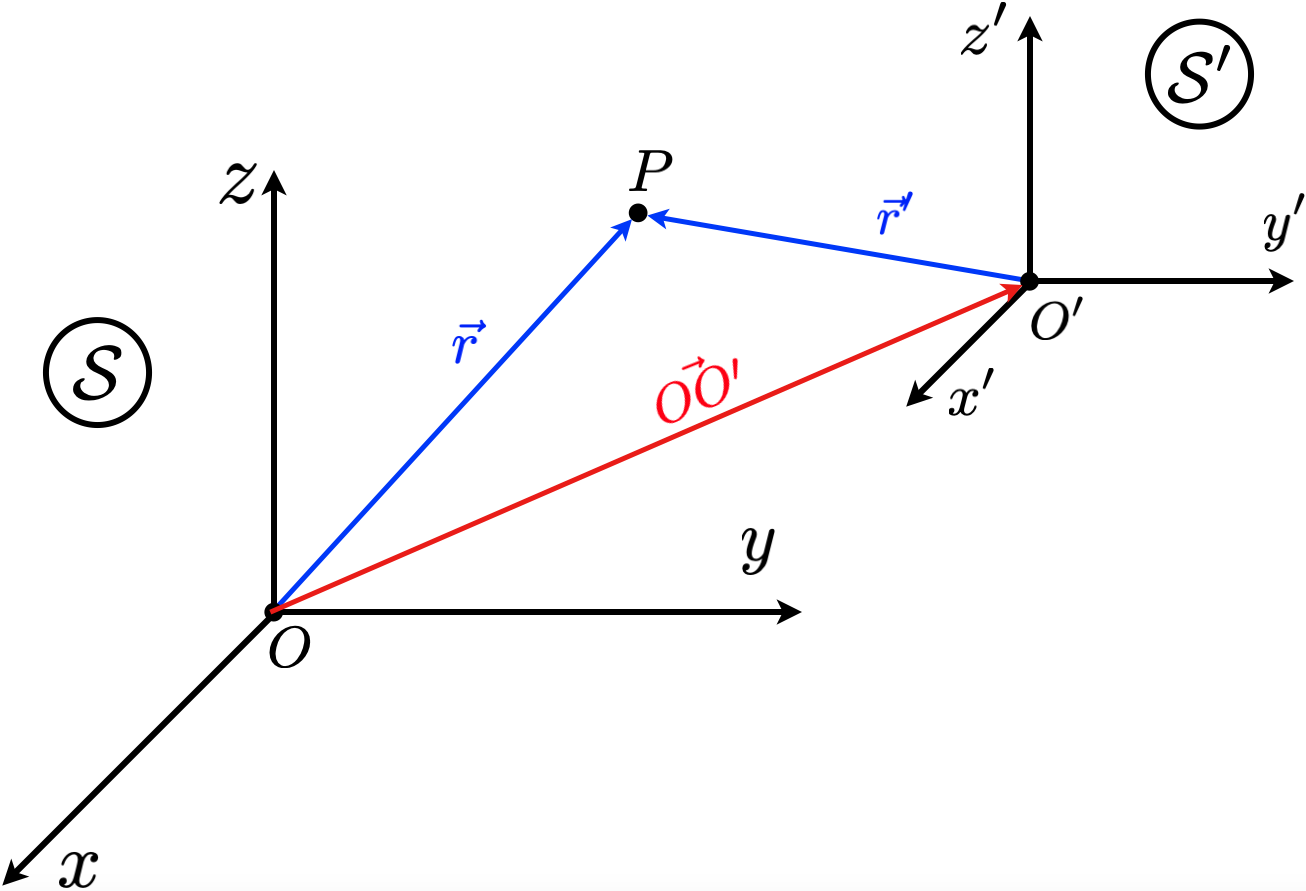
\includegraphics[width=13cm]{images/relativemotions.png}
    \caption{Rappresentazione del sistema di riferimento fisso $\mathcal{S}$,
    e del sistema  $\mathcal{S'}$ in moto generico rispetto ad  $\mathcal{S}$.}
\label{fig:RelativeMotions}
\end{figure}
Il concetto di moto relativo è cruciale in fisica. Di conseguenza dobbiamo
disporre di alcune formule che trasformano le grandezze misurate in un dato
sistema di riferimento in quelle misurare in un altro sistema, in moto
rispetto al primo.\\
Vedremo quindi come le posizioni, le velocità e le accelerazioni trasformano
da un sistema all'altro. Questi concetti sono ben noti fin dal 1600, e la
teoria che vedremo è chiamata relatività galileiana.\\
Nella relatività galileliana, a differenza della relatività speciale di
Einstein, il tempo è assoluto, ovvero scorre nello stesso identico modo per
ogni osservatore.
Di conseguenza gli eventi in questo spazio-tempo, saranno identificati dallo
stesso parametro temporale $t$ e dai vettori $\vec r$ ed $\vec r'$.

\section{Teorema delle velocità relative}

Dati due differenti sistemi di riferimento,  $\mathcal{S}$ in quiete, ed
$\mathcal{S'}$ in moto rispetto ad  $\mathcal{S}$, si vogliono trovare le
relazioni che legano le grandezze osservate nel sistema fisso e quelle
osservate nel sistema mobile.\\
Quindi preso un punto generico $P$ nello spazio, esso avrà come raggio
vettore $\vec r$ in  $\mathcal{S}$, ed $\vec r'$ in  $\mathcal{S'}$.
\\Possiamo dunque scrivere che:

\begin{equation}
    \vec r - \vec{OO'} = \vec r' \seg \boxed{ \vec r' = \vec r - \vec r_{0(t)}}
\label{eq:r_prime}
\end{equation}
\\
Dove $\vec{OO'}$, chiamato d'ora in poi $\vec r_{0(t)}$, è il raggio vettore
dell'origine del sistema $\mathcal{S'}$.
Derivando rispetto al tempo l'equazione (\ref{eq:r_prime}) si otterrà la
velocità del punto $P$ nel sistema $\mathcal{S'}$ in funzione della velocità
in $\mathcal{S}$, della velocità di traslazione del sistema $\mathcal{S'}$
ed in generale anche della velocità angolare con cui ruota $\mathcal{S'}$.

\begin{equation}
    \frac{d\vec r'}{dt} = \frac{d\vec r}{dt} - \frac{d\vec r_0}{dt}
\end{equation}
\\
Definiamo con $\vec u = \frac{d\vec r_0}{dt}$ la veloctià dell'origine $O'$,
mentre dato che $\vec r' = x'\hat u_{x'} + y'\hat u_{y'} + z'\hat u_{z'}$,
occorre derivare anche i versori direzionali del sistema $\mathcal{S'}$.

\begin{equation}
    \frac{d\vec r'}{dt} = \dot x'\hat u_{x'}+\dot y'\hat u_{y'}+\dot z'\hat u_{z'}+
    + x'\frac{d\hat u_{x'}}{dt}+ y'\frac{d\hat u_{y'}}{dt}+ z'\frac{d\hat u_{z'}}{dt}
    =\vec v-\vec u
\end{equation}
\\
Quindi definendo $\vec v' = \dot x'\hat u_{x'}+\dot y'\hat u_{y'}+
\dot z'\hat u_{z'}$ e ricordando che $\frac{d\hat u_{x'_i}}{dt} =
\vec\omega\times\hat u_{x'_i}$ otterremo il teorema delle velocità relative:

\begin{equation}
    \boxed{\vec v' = \vec v - \vec u - \vec \omega\times\vec r'}
\end{equation}
\\
\begin{equation}
    \vec v_t \coloneqq \vec v - \vec v' = \vec u + \vec \omega\times\vec r'
    \seg \boxed{\vec v' = \vec v - \vec v_t}
\end{equation}
\section{Teorema delle accelerazioni relative}
%--------------------------------------------------------------------------
Analogamente al caso delle velocità se definiamo $\vec a_0 = \frac{d\vec u}{dt}$
ed $\vec a' = \ddot x'\hat u_{x'}+\ddot y'\hat u_{y'}+\ddot z'\hat u_{z'}$
possiamo scrivere che:

\begin{equation}
    \frac{d\vec v'}{dt} = \vec a' + \vec\omega\times\vec v' = \vec a - \vec a_0
    -\frac d{dt}\sx\vec\omega\times\vec r'\dx
\end{equation}
\\
\begin{equation}
    \frac d{dt}\sx\vec\omega\times\vec r'\dx = \frac{d\vec\omega}{dt}\times\vec r'
    + \vec\omega\times\frac{d\vec r'}{dt} = \vec\alpha\times\vec r' + \vec\omega\times
    \sx\vec v' + \vec\omega\times\vec r'\dx
\end{equation}
\\
\begin{equation}
    \boxed{\vec a' = \vec a - \vec a_0 - 2\vec\omega\times\vec v'-\vec\alpha\times
    \vec r' - \vec\omega\times\vec\omega\times\vec r'}
\end{equation}
\\
In questo caso l'accelerazione di trascinamento è definita come $\vec a_t = 
\vec a_0 + \vec\alpha\times\vec r' +\vec\omega\times\vec\omega\times\vec r'$,
quindi in definitiva avremo che:

\begin{equation}
    \vec a' = \vec a - \vec a_t -2\vec\omega\times\vec v'
\end{equation}
\\
Abbiamo quindi disaccoppiato da $\vec a_t$ un termine dipendente dalla velocità
del punto in $\mathcal{S'}$, chiamato accelerazione di Coriolis.

\begin{equation}
    \vec a_{cor} = 2\vec\omega\times\vec v'\seg \boxed{\vec a' = \vec a -\vec a_t
    -\vec a_{cor}}
\end{equation}
\section{Sistemi inerziali e non inerziali}
%---------------------------------------------------------------------------
Possiamo classificare i sistemi di riferimento in due macrogruppi: inerziali
e non inerziali.\\
Un sistema è detto inerziale se in assenza di forze esterne applicate un corpo
si muove di moto rettilineo uniforme. Ovvero vale il primo principio della
dinamica e di conseguenza un sistema è inerziale rispetto ad un altro se si
muove di moto rettilineo uniforme rispetto a quest'ultimo.\\
Tutti i sistemi che non rispettano queste condizioni sono detti non inerziali.

\subsection{Inerziali}

Se $\vec r_{0(t)} = \vec r_0 + \vec u t$ avremo che $\vec a_0 = \vec0$ ed
anche $\vec\omega = \vec 0$, quindi la velocità e l'accelerazione misurate
in $\mathcal{S'}$ saranno:

\begin{equation}
    \vec v' = \vec v - \vec u \seg \vec a' = \vec a
\end{equation}
\\
Tra sistemi inerziali dunque, le velocità di sottraggono mentre le accelerazioni
sono le stesse, ne segue che anche le forze sono le stesse.

\begin{equation}
    \vec F = m\vec a\qquad \vec F' = m\vec a' = m\vec a = \vec F
\end{equation}
\\
Concludiamo quindi che i sistemi di riferimento inerziali sono equivalenti dal
punto di vista meccanico, e non esistono dunque esperimenti che possono indicare
quale de due sistemi sia in movimento.

\subsection{Non inerziali}

Nei sistemi non ineziali troveremo $\vec a_t \ne \vec0$ e/o $\vec\omega \ne \vec 0$,
quindi $\vec a' = \vec a$.

\begin{equation}
        \vec F' = m\vec a' = m\vec a -m\vec a_t - m\vec a_{cor} = \vec F -
        \vec F_t -\vec F_{cor}
\end{equation}
\\
Come possiamo notare anche in assenza di forze esterne applicate, con
$\vec F = \vec 0$, si avrà $\vec F' = - \vec F_t -\vec F_{cor}$. Compaiono
quindi le forze inerziali che alterano apparentemente il moto rettilineo
uniforme degli oggetti.
\section{Esempi di trasformazioni}
%---------------------------------------------------------------------------
Vediamo ora qualche trasformazione nota, nel caso in cui le due origini dei
sistemi all'inizio dei tempi coincidano. Studieremo i tre casi di moto rettilineo
uniforme, uniformemente accelerato e circolare.

\subsection{Moto rettilineo uniforme}

\begin{equation}
    \vec r_{0(t)} = \vec v_0 t\qquad \vec v_0 = v_0\hat u_x
\end{equation}
\\
\begin{equation}
    \begin{cases}
        x' = x - v_0t\\
        y' = y\\
        z' = z
    \end{cases}\seg
    \begin{cases}
        v_x' = v_x - v_0\\
        v_y' = v_y\\
        v_z' = v_z
    \end{cases}
\end{equation}

\subsection{Moto rettilineo uniformemente accelerato}

\begin{equation}
    \vec r_{0(t)} = \frac12\vec a_0 t^2\qquad \vec v_{0(t)} = \vec a_0t
    \qquad \vec a_0 = a_0\hat u_x
\end{equation}
\\
\begin{equation}
    \begin{cases}
        x' = x - \frac12a_0t^2\\
        y' = y\\
        z' = z
    \end{cases}\seg
    \begin{cases}
        v_x' = v_x - a_0t\\
        v_y' = v_y\\
        v_z' = v_z
    \end{cases}\seg
    \begin{cases}
        a_x' = a_x - a_0\\
        a_y' = a_y\\
        a_z' = a_z
    \end{cases}
\end{equation}

\subsection{Moto circolare uniforme}

\begin{equation}
    \vec r_0 = \vec v_0 = \vec a_0 = \vec0
    \qquad \vec\omega = \omega_0\hat u_z
    \seg
    \begin{cases}
        \vec r' = \vec r\\
        \vec v' = \vec v - \vec\omega\times\vec r'\\
        \vec a' = \vec a - 2\vec\omega\times\vec v' -\vec\omega\times\vec\omega
        \times\vec r'
    \end{cases}
\end{equation}
\\
Quindi anche considerando un punto fermo, ovvero con $\vec v = \vec 0$, quindi
anche $\vec a = \vec 0$. Ne segue che:

\begin{equation}
    \begin{cases}
        \vec v' = - \vec\omega\times\vec r\\
        \vec a' = - 2\vec\omega\times\vec v' -\vec\omega\times\vec\omega
        \times\vec r = \vec\omega\times\vec\omega\times\vec r = 
        \sx\vec\omega\cdot\vec r\dx\vec\omega -\omega^2\vec r
    \end{cases}
\end{equation}
\\
Dato che $\vec\omega\perp\vec r$ otteniamo $\vec a' = -\omega^2\vec r$. Come
è giusto che sia, in $\mathcal{S'}$ il punto fermo in $\vec r$ appare ruotare
in direzione opposta alla quella attorna alla quale in realtà sta ruodando il
sistema, dunque si misura una forza apparente pari appunto alla forza centripeta.

